\documentclass[sigconf,nonacm]{acmart}

\settopmatter{printacmref=false}
\renewcommand\footnotetextcopyrightpermission[1]{}
\pagestyle{plain}

\usepackage{booktabs}
\usepackage{array}
\usepackage{graphicx}

\title{Attack-Type-Specific Evaluation of Neural and Traditional Models for Flow-Level Intrusion Detection}

\author{Yonghyeon Lee}
\email{yhylee@ucdavis.edu}
\affiliation{%
  \country{}
}

\begin{abstract}
Network intrusion detection studies often compare models using aggregate metrics such as precision, recall, or F1-score.
These metrics are useful for high-level comparison, but they compress heterogeneous attack behavior into a single score and can hide which attack types remain uncovered.
In particular, strong performance on easier high-signal attacks can make a model appear reliable overall, while false negatives on rare, stealthy, or operationally important attacks remain buried in the average.
This paper uses the comparison between neural and traditional machine learning models as an experimental lens to study this limitation in flow-level intrusion detection.
Using the CSE-CIC-IDS2018 processed flow-feature dataset, I train Logistic Regression, Random Forest, Shallow MLP, Lightweight PyTorch MLP, Deep MLP, and Autoencoder + MLP on the same binary benign/malicious task while preserving original attack labels for post-hoc attack-type analysis.
The results show that aggregate metrics and attack-type-specific false negatives can support different model choices: Deep MLP and Autoencoder + MLP improve precision and F1-score, while Logistic Regression has the highest attack recall and lowest false-negative rate.
Attack-type analysis further shows that DoS/DDoS and many brute-force attacks are detected well, Random Forest is strongest on Bot and SQL Injection, and Infiltration remains a shared blind spot for every model.
These findings suggest that attack-type-specific analysis is not only an interpretive add-on, but a practical evaluation step for choosing models, tuning thresholds, and designing more flexible hybrid IDS systems around the attack families each model covers best.
IDS evaluation should therefore combine aggregate metrics with attack-type-specific false-negative analysis so future IDS designs can make more diverse, coverage-oriented choices instead of selecting one global winner.
\end{abstract}

\keywords{intrusion detection, neural networks, Random Forest, false negatives, CSE-CIC-IDS2018, attack-type evaluation}

\begin{document}
\maketitle

\section{Introduction}

Network intrusion detection systems classify network activity as benign or suspicious so that defenders can investigate or block malicious traffic.
In many machine learning studies of intrusion detection, the headline result is an aggregate score such as accuracy or F1-score.
That style of reporting is useful for comparing models at a high level, but it is incomplete for security analysis.
In an operational IDS, different mistakes have different costs.
A false positive creates analyst workload, but a false negative means malicious traffic passed through without being flagged.
Even if a model has a strong aggregate score, it may still systematically miss an attack family that is operationally important.

This project studies that problem in the setting of flow-level intrusion detection.
Flow-level datasets summarize network traffic using features such as packet counts, byte counts, flow duration, rates, inter-arrival timing, and TCP flag behavior.
These features are much easier to use in a quarter-scale reproducible study than raw packet traces, and they support both traditional machine learning and neural network models.
At the same time, flow-level data has a risk: aggregate binary classification can hide large differences across attack categories.
The central problem is whether aggregate IDS metrics can make a model look strong while hiding attack types that remain poorly covered.

This leads to the research question:
\emph{what limitations do aggregate metrics have when evaluating flow-level IDS models, and how can those limitations be complemented?}
This question is not a leaderboard-style search for the best IDS model.
Instead, the neural/traditional comparison is used as an experimental lens for studying whether strong aggregate scores can coexist with weak coverage of operationally important attack types.
More specifically, the project examines DoS/DDoS, brute force, botnet, infiltration, and web-based attacks to identify where each model succeeds, where it fails, and whether those attack-type results can guide model selection, debugging, or future hybrid IDS design.

I hypothesized that aggregate metrics would not fully reflect the security coverage of each model.
More specifically, I expected neural models to improve some aggregate scores and some attack categories whose signatures depend on nonlinear combinations of flow-level features, such as botnet or web-based traffic.
At the same time, I expected traditional models, especially Random Forest, to remain competitive on attacks with clearer separable feature patterns, such as high-volume DDoS traffic.
The broader hypothesis is that different model families would leave different attack-type blind spots, so attack-type-specific false-negative analysis would reveal security-relevant differences hidden by aggregate metrics.

The theoretical contribution of this work is an attack-type-specific evaluation framework for showing how aggregate IDS metrics can hide security-relevant false negatives.
Rather than summarizing model behavior with one aggregate score, the framework compares which attack types each model detects and which attack types it leaves uncovered.
In this framing, model comparison is not only a ranking exercise, but also a diagnostic procedure for identifying which traffic patterns each model family is strong or weak at detecting.
The empirical contribution is a reproducible implementation that trains Logistic Regression, Random Forest, Shallow MLP, Lightweight PyTorch MLP, Deep MLP, and Autoencoder + MLP on the same CSE-CIC-IDS2018 sample and reports both model-level and attack-level false negatives.
The final result shows that neural models can improve some aggregate metrics, but they do not consistently reduce missed attacks, and important blind spots such as Infiltration are not visible from aggregate scores alone.

\section{Related Work}

Prior work on intrusion detection datasets motivates the empirical setting of this project.
CICIDS2017 was introduced to provide a more realistic benchmark than older IDS datasets.
It includes benign traffic and common attack traffic represented through labeled network-flow features [1].
CSE-CIC-IDS2018 extends this direction with a larger cyber-defense dataset containing multiple attack scenarios, including brute force, Heartbleed, botnet, DoS, DDoS, web attacks, and infiltration [2].
These datasets are directly relevant because they support both binary benign/malicious detection and attack-category-specific analysis.
In this paper, CSE-CIC-IDS2018 is especially useful because the models are trained on a binary IDS task while the original attack labels are preserved for post-hoc analysis.

Prior work on IDS modeling motivates the model set used in this study.
Logistic Regression provides a simple linear baseline, while Random Forest is a standard traditional machine learning baseline because it combines many decision-tree predictors into an ensemble [3].
Deep learning has also been studied for network intrusion detection.
Gamage and Samarabandu survey deep learning approaches for IDS and compare feed-forward neural networks, autoencoders, deep belief networks, and LSTMs on legacy and modern IDS datasets [4].
More specifically, Rosay, Carlier, and Leroux propose an MLP-based intrusion detection system for the CICIDS2017 dataset and report that a carefully designed MLP can be competitive with traditional machine learning techniques [5].
Song, Hyun, and Cheong analyze autoencoders for network intrusion detection and show that autoencoder design choices such as model capacity, latent size, and thresholding can strongly affect IDS performance [6].
These studies support the inclusion of MLP-based neural models and an autoencoder-based representation-learning model.
At the same time, prior work also shows that simply adding a neural architecture is not a new contribution by itself.

The gap this project addresses is in how IDS model performance is interpreted.
Many IDS studies emphasize overall accuracy or aggregate detection performance [4], but aggregate metrics can hide security-relevant failures when datasets are imbalanced or when some attack categories are harder to detect.
Saito and Rehmsmeier show that precision-recall analysis is especially informative for imbalanced classification problems [7].
This matters for IDS because a false negative represents malicious traffic that the system fails to flag.
For that reason, this paper treats recall, false-negative rate, and attack-type detection rate as central security metrics rather than as secondary diagnostics.

Therefore, this project fits within existing work but asks a narrower and more security-centered question.
It does not claim that neural models simply perform IDS better than traditional machine learning.
Instead, it compares Logistic Regression, Random Forest, Shallow MLP, Lightweight PyTorch MLP, Deep MLP, and Autoencoder + MLP models under the same flow-level pipeline to identify which attack categories each model misses.
The neural and traditional baselines are therefore not used to claim a new best IDS architecture, but to examine whether common model-comparison metrics obscure attack-specific failure modes.
This framing matches the final experimental goal: neural models may improve precision or F1-score, but the more important security question is whether they reduce missed attacks across DoS/DDoS, brute force, botnet, infiltration, and web attack categories.
The related work supports the project in three ways: CICIDS datasets provide the labeled flow-level setting, prior ML/DL IDS work justifies the model comparison, and imbalanced-evaluation research motivates using attack-type recall and false-negative analysis to complement aggregate metrics.

\section{Method}

\subsection{Dataset and Filtering}

The study uses the CSE-CIC-IDS2018 processed traffic data for machine learning.
The raw files were downloaded from the public AWS S3 bucket and processed into a reproducible sampled dataset.
The final sample contains 50,000 flows, 79 numeric flow features, 37,308 benign flows, and 12,692 attack flows.
The preprocessing step preserves 14 fine-grained attack labels so that binary model outputs can later be analyzed by attack type.

The task used for model training is binary classification.
Each row is labeled as benign or malicious.
The original attack label is not used as the prediction target, because the research question is about whether aggregate binary IDS metrics hide different attack-type failures.
Instead, the original label is carried through the train, validation, and test split and used only for post-hoc evaluation.

The preprocessing pipeline cleans column names, detects the label column, removes non-feature metadata columns, replaces missing and infinite values, scales numeric features, and splits the data into training, validation, and test sets.
The final split contains 32,000 training rows, 8,000 validation rows, and 10,000 test rows.
The random seed is fixed at 42 for reproducibility.
Rare-label preservation is used during sampling so that small attack categories are not accidentally removed.

\subsection{System Building Blocks}

The implemented system is a lightweight flow-level IDS prototype.
It has four main building blocks.
First, the dataset preparation script downloads or reads raw CSE-CIC-IDS2018 CSV files, samples rows while preserving attack labels, and writes a processed training CSV.
Second, the training pipeline loads the processed CSV, applies the shared preprocessing pipeline, trains all selected models, and saves model artifacts.
Third, the evaluation module generates binary metrics, attack-type detection summaries, attack-family detection summaries, and plots.
Fourth, the prediction module loads saved artifacts and applies a trained model to a new CSV file.

The system is implemented in Python using pandas, NumPy, scikit-learn, PyTorch, and matplotlib.
scikit-learn is used for Logistic Regression, Random Forest, scaling, splitting, and metric computation.
PyTorch is used for the neural models and training loops.
The repository also includes a README with commands for reproducing data preparation, training, and prediction.

\subsection{Models}

Six models are compared.
The six models vary in complexity and inductive bias so the experiment can test whether different aggregate scores correspond to different attack-type blind spots.
Logistic Regression is the simple linear baseline and uses balanced class weights.
Random Forest is the traditional non-neural baseline and uses balanced subsampling.
The neural baselines are Shallow MLP, Lightweight PyTorch MLP, Deep MLP, and Autoencoder + MLP.
The Shallow MLP has one hidden layer.
The Lightweight PyTorch MLP is the original two-hidden-layer model.
The Deep MLP uses more feed-forward layers to test whether depth improves attack recall.
The Autoencoder + MLP first learns a compressed latent representation and then feeds that representation to a classifier.

All models are trained and evaluated on the same split.
This keeps the comparison focused on model behavior rather than data differences.
The neural models are not heavily tuned, because the goal is a scoped comparison of attack-specific failure patterns rather than a leaderboard-style optimization.

\subsection{Measures}

The main metrics are precision, recall, F1-score, false-negative rate, attack-type detection rate, and attack-family detection rate.
For the binary malicious class, recall measures the fraction of attacks detected.
False-negative rate is one minus recall and directly measures the fraction of attacks missed.
Precision measures how many flows predicted as malicious were actually malicious.
F1-score balances precision and recall.
Let TP, FP, and FN denote true positives, false positives, and false negatives for the malicious class.
The aggregate metrics are computed as:
\begin{equation}
\begin{aligned}
\mathrm{Precision} &= \frac{TP}{TP + FP}, \\
\mathrm{Recall} &= \frac{TP}{TP + FN}, \\
\mathrm{F1} &= \frac{2 \cdot \mathrm{Precision} \cdot \mathrm{Recall}}
{\mathrm{Precision} + \mathrm{Recall}}, \\
\mathrm{FNR} &= \frac{FN}{TP + FN} = 1 - \mathrm{Recall}.
\end{aligned}
\end{equation}

Attack-type detection rate is computed by grouping malicious test rows by their original fine-grained attack label and measuring the fraction of rows detected as malicious by each model.
Attack-family detection rate maps fine-grained labels into five broader groups: Botnet, Brute Force, DoS/DDoS, Infiltration, and Web Attack.
These two levels of analysis are both necessary.
The fine-grained view shows specific failure cases, while the family-level view summarizes broader security patterns.
Together, these group-level metrics complement aggregate precision, recall, and F1-score by showing which attack categories remain uncovered.
For an attack type or family \(g\), the group detection rate is:
\begin{equation}
\mathrm{DetectionRate}(g) =
\frac{\sum_{i \in G_g} \mathbf{1}[\hat{y}_i = 1]}
{|G_g|},
\end{equation}
where \(G_g\) is the set of malicious test flows whose original label belongs to group \(g\), and \(\hat{y}_i=1\) means the model predicted flow \(i\) as malicious.

\subsection{Implementation and Reproducibility}

The experiment was executed as a reproducible command-line pipeline rather than as a manually edited notebook.
This matters because the project compares several models and many attack categories; manual steps would make it easy to accidentally evaluate different models on different splits.
The repository contains separate scripts for dataset preparation, training, evaluation, and prediction.
The dataset preparation command reads the raw CSE-CIC-IDS2018 CSV files, applies rare-label-preserving sampling, and writes a processed CSV.
The training command then reads that processed file, creates the fixed train/validation/test split, trains all models, saves artifacts, and writes result tables and plots.

The final execution used the CSE-CIC-IDS2018 processed machine-learning CSV files downloaded from the public AWS bucket.
The raw local dataset contained 10 CSV files totaling about 6.41 GB.
The processed experiment sample was saved as \texttt{data/processed/ids\_sample.csv}.
The run produced model artifacts for Logistic Regression, Random Forest, Shallow MLP, PyTorch MLP, Deep MLP, and Autoencoder + MLP.
It also produced \texttt{metrics\_summary.csv}, \texttt{attack\_type\_detection.csv}, \texttt{attack\_family\_detection.csv}, false-negative plots, and prediction outputs.
These outputs provide evidence that the project was executed according to the planned method: the same dataset split was used across models, attack labels were preserved for evaluation, and both aggregate and attack-specific results were collected.
The prediction script can also load a saved model and apply it to a CSV file, which demonstrates the system-building component beyond offline reporting.

\section{Results}

\subsection{Overall Model Performance}

Table~\ref{tab:overall} reports binary malicious-class performance on the 10,000-row test split.
This table illustrates the central tension of the study: the aggregate F1-score favors Deep MLP, while the security-focused false-negative metrics favor Logistic Regression.
Deep MLP achieves the highest F1-score and precision.
However, Logistic Regression achieves the highest recall and the lowest false-negative rate.
This distinction is central to the security interpretation of the experiment.
The model that looks best by F1-score is not the model that misses the fewest attacks.

\begin{table}[t]
  \caption{Overall malicious-class performance on the test split.}
  \label{tab:overall}
  \centering
  \small
  \begin{tabular}{lrrrr}
    \toprule
    Model & Precision & Recall & F1 & FNR \\
    \midrule
    Logistic Regression & 0.512 & 0.528 & 0.520 & 0.472 \\
    Random Forest & 0.649 & 0.471 & 0.546 & 0.529 \\
    Shallow MLP & 0.578 & 0.524 & 0.550 & 0.476 \\
    PyTorch MLP & 0.615 & 0.507 & 0.556 & 0.493 \\
    Deep MLP & 0.747 & 0.467 & 0.574 & 0.533 \\
    Autoencoder + MLP & 0.723 & 0.471 & 0.570 & 0.529 \\
    \bottomrule
  \end{tabular}
\end{table}

\paragraph{Logistic Regression.}
Logistic Regression has the highest recall (0.528) and the lowest false-negative rate (0.472), missing 1,197 attacks.
It is the weakest model by precision, but it is the safest model in this experiment if the priority is to minimize missed malicious flows.

\paragraph{Random Forest.}
Random Forest improves precision to 0.649, but its recall falls to 0.471 and it misses 1,342 attacks.
This suggests that the tree ensemble is more selective than Logistic Regression at the binary level, even though later attack-type results show that it is strong on Botnet and Web Attack.

\paragraph{Shallow MLP.}
Shallow MLP is the strongest neural model by recall, with 0.524 recall and 1,209 missed attacks.
Its behavior is close to Logistic Regression, but with better precision and F1-score, making it the most balanced neural baseline.

\paragraph{Lightweight PyTorch MLP.}
The two-hidden-layer PyTorch MLP improves precision and F1-score relative to Logistic Regression, but recall drops to 0.507 and false negatives increase to 1,252.
It therefore offers a moderate precision-recall tradeoff rather than a clear reduction in missed attacks.

\paragraph{Deep MLP.}
Deep MLP has the highest precision (0.747) and F1-score (0.574), but also the highest false-negative rate (0.533) and 1,354 missed attacks.
It is the most selective model: when it predicts malicious, it is often correct, but it leaves more attacks undetected.

\paragraph{Autoencoder + MLP.}
Autoencoder + MLP behaves similarly to Deep MLP, with high precision (0.723), high F1-score (0.570), and a high false-negative rate (0.529).
The learned representation improves selectivity but does not solve the IDS recall problem.

\begin{figure}[t]
  \centering
  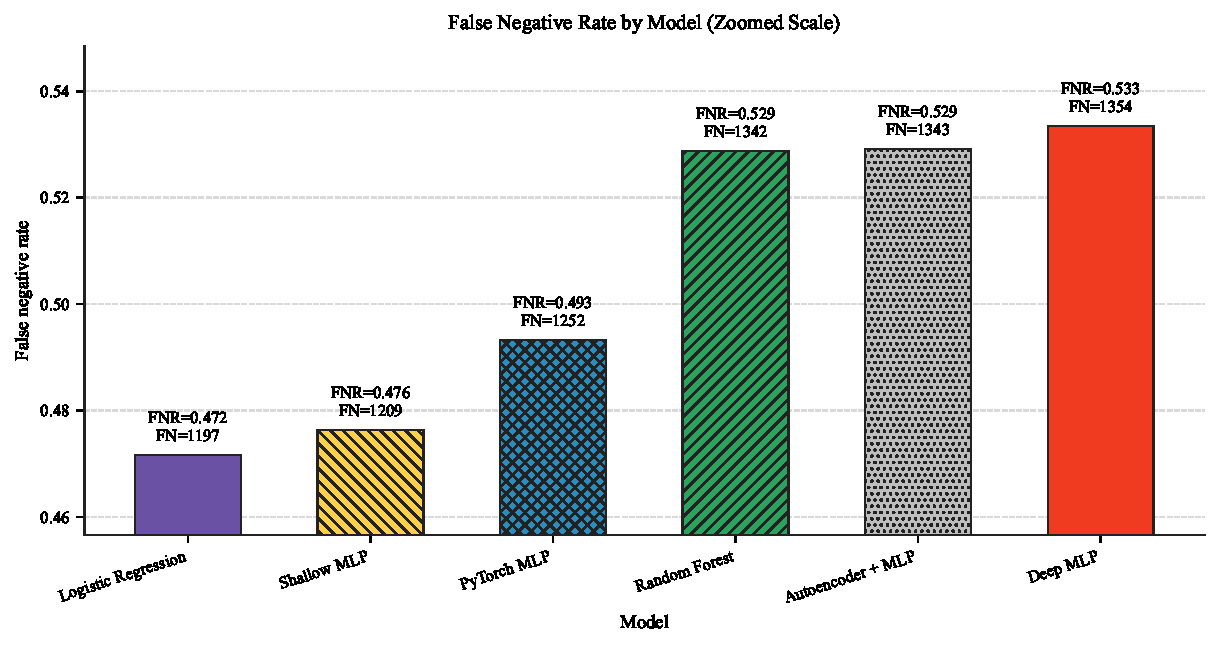
\includegraphics[width=\linewidth]{reports/final_run/false_negative_rate.pdf}
  \caption{False-negative rate by model on a zoomed y-axis. Lower is better for IDS security coverage.}
  \Description{Zoomed bar chart comparing false-negative rate and false-negative count across the six evaluated models.}
  \label{fig:fnr}
\end{figure}

\subsection{Coarse Attack-Family Results}

Table~\ref{tab:families} summarizes the strongest model for each coarse attack family.
The family-level results show why aggregate metrics need attack-type context: the difficulty of the IDS task depends strongly on the attack family.
DoS/DDoS is nearly solved by the tested models.
Shallow MLP and PyTorch MLP both reach 1.000 recall on the DoS/DDoS family.
Random Forest is strongest on Botnet and Web Attack.
For Brute Force, Random Forest, Shallow MLP, and PyTorch MLP tie at 0.932 recall.

\begin{table}[t]
  \caption{Best model by coarse attack-family recall.}
  \label{tab:families}
  \centering
  \small
  \begin{tabular}{lll}
    \toprule
    Family & Best model & Recall \\
    \midrule
    Botnet & Random Forest & 0.958 \\
    Brute Force & RF / Shallow MLP / PyTorch MLP & 0.932 \\
    DoS/DDoS & Shallow MLP / PyTorch MLP & 1.000 \\
    Infiltration & Logistic Regression & 0.299 \\
    Web Attack & Random Forest & 1.000 \\
    \bottomrule
  \end{tabular}
\end{table}

The most important result is the Infiltration family.
It has 1,669 test attacks, but even the best model, Logistic Regression, detects only 499 of them.
The family-level recall is only 0.299.
Random Forest detects 334, Shallow MLP detects 469, PyTorch MLP detects 428, Deep MLP detects 359, and Autoencoder + MLP detects 367.
This family drives a large portion of the overall false negatives.

\begin{figure}[t]
  \centering
  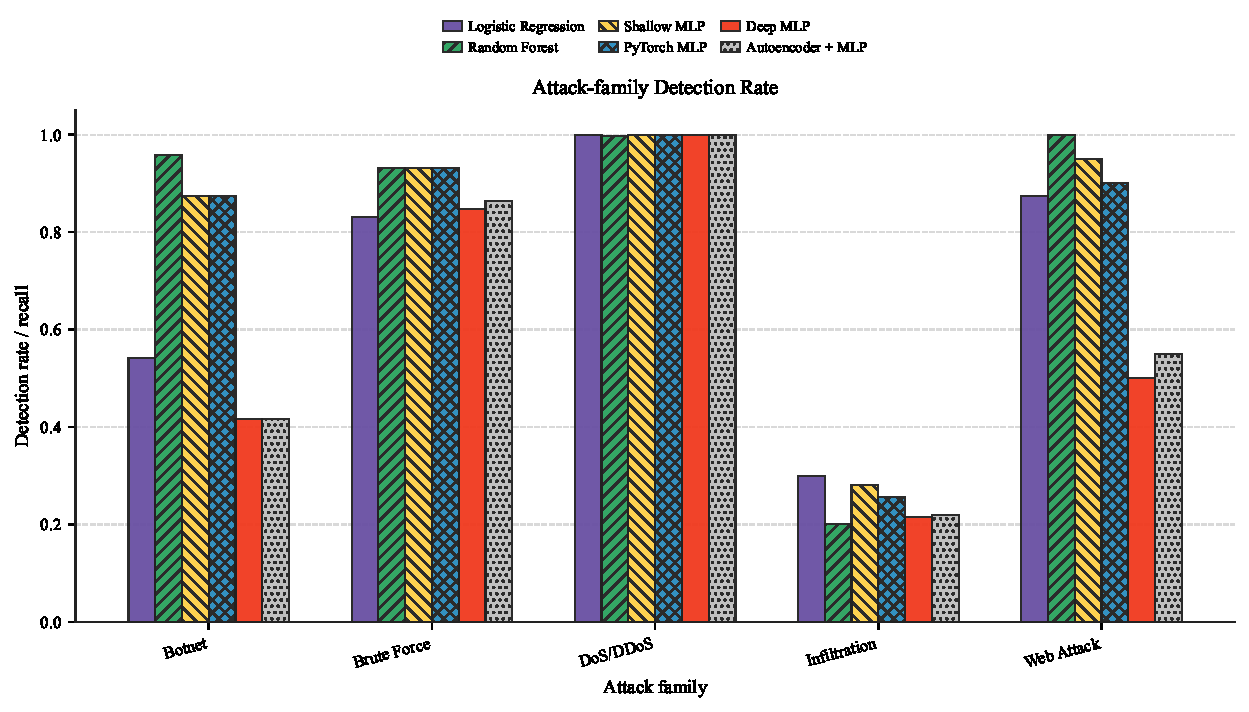
\includegraphics[width=\linewidth]{reports/final_run/attack_family_detection.pdf}
  \caption{Detection recall by coarse attack family and model.}
  \Description{Grouped bar chart showing recall by coarse attack family for each model.}
  \label{fig:family}
\end{figure}

\subsection{Fine-Grained Attack-Type Results}

The fine-grained results explain which specific attacks create the family-level patterns.
They also show the concrete failure modes that aggregate model scores compress into a single number.
Several attack labels are detected almost perfectly by nearly all models.
DDOS attack-HOIC, DDOS attack-LOIC-UDP, DoS attacks-SlowHTTPTest, FTP-BruteForce, and SSH-Bruteforce all have near-perfect or perfect recall across most models.
These attacks appear to have flow-feature signatures that are easier to separate from benign traffic.

Table~\ref{tab:finegrained} reports the per-label recall values used for this analysis.
The table is useful because the best model changes by attack type.
It also shows that the headline difficulty is not evenly distributed across the dataset.
Some rows are almost entirely solved, while Infilteration remains consistently weak across all six models.

\begin{table}[t]
  \caption{Fine-grained attack-type recall by model. LR = Logistic Regression, RF = Random Forest, Shallow = Shallow MLP, PT = PyTorch MLP, Deep = Deep MLP, AE = Autoencoder + MLP.}
  \label{tab:finegrained}
  \centering
  \scriptsize
  \setlength{\tabcolsep}{2pt}
  \resizebox{\columnwidth}{!}{%
  \begin{tabular}{lrrrrrrr}
    \toprule
    Attack type & Test & LR & RF & Shallow & PT & Deep & AE \\
    \midrule
    Bot & 24 & 0.542 & 0.958 & 0.875 & 0.875 & 0.417 & 0.417 \\
    Brute Force -Web & 18 & 0.444 & 0.778 & 0.778 & 0.778 & 0.500 & 0.556 \\
    Brute Force -XSS & 20 & 1.000 & 1.000 & 1.000 & 1.000 & 0.450 & 0.450 \\
    DDOS attack-HOIC & 618 & 1.000 & 1.000 & 1.000 & 1.000 & 1.000 & 1.000 \\
    DDOS attack-LOIC-UDP & 15 & 1.000 & 1.000 & 1.000 & 1.000 & 1.000 & 1.000 \\
    DDoS attacks-LOIC-HTTP & 20 & 0.950 & 0.950 & 1.000 & 1.000 & 1.000 & 1.000 \\
    DoS attacks-GoldenEye & 19 & 1.000 & 1.000 & 1.000 & 1.000 & 0.947 & 1.000 \\
    DoS attacks-Hulk & 23 & 1.000 & 0.957 & 1.000 & 1.000 & 1.000 & 1.000 \\
    DoS attacks-SlowHTTPTest & 28 & 1.000 & 1.000 & 1.000 & 1.000 & 1.000 & 1.000 \\
    DoS attacks-Slowloris & 23 & 1.000 & 1.000 & 1.000 & 1.000 & 1.000 & 0.957 \\
    FTP-BruteForce & 18 & 1.000 & 1.000 & 1.000 & 1.000 & 1.000 & 1.000 \\
    Infilteration & 1669 & 0.299 & 0.200 & 0.281 & 0.256 & 0.215 & 0.220 \\
    SQL Injection & 20 & 0.750 & 1.000 & 0.900 & 0.800 & 0.550 & 0.650 \\
    SSH-Bruteforce & 23 & 1.000 & 1.000 & 1.000 & 1.000 & 1.000 & 1.000 \\
    \bottomrule
  \end{tabular}
  }
\end{table}

\paragraph{DDoS attacks-LOIC-HTTP.}
DDoS attacks-LOIC-HTTP is one case where the neural models are slightly more stable.
Shallow MLP, PyTorch MLP, Deep MLP, and Autoencoder + MLP all achieve 1.000 recall, while Logistic Regression and Random Forest each miss one sample.
This supports the hypothesis in a limited sense: there are some attack types where neural models match or slightly improve the traditional baselines.

\paragraph{Bot.}
Bot traffic shows the opposite pattern.
Random Forest reaches 0.958 recall, while Logistic Regression reaches 0.542 and the deeper neural models perform poorly.
Deep MLP and Autoencoder + MLP each reach only 0.417 recall on Bot.
This suggests that a tree-based model may capture useful feature thresholds for this small category better than the deeper neural models used in this experiment.

\paragraph{Brute Force -Web.}
Brute Force -Web also favors models that can represent feature interactions.
Random Forest, Shallow MLP, and PyTorch MLP all reach 0.778 recall, while Logistic Regression reaches 0.444.
\paragraph{Brute Force -XSS.}
Brute Force -XSS shows that deeper neural models are not automatically more robust on rare labels.
Logistic Regression, Random Forest, Shallow MLP, and PyTorch MLP reach 1.000 recall, but Deep MLP and Autoencoder + MLP reach only 0.450.

\paragraph{SQL Injection.}
SQL Injection is strongest under Random Forest, which reaches 1.000 recall.
Shallow MLP is also strong at 0.900, while Logistic Regression reaches 0.750, PyTorch MLP reaches 0.800, Deep MLP reaches 0.550, and Autoencoder + MLP reaches 0.650.
This supports the broader result that Random Forest remains competitive and sometimes superior for web-related attacks.

\paragraph{Infilteration.}
The most important fine-grained attack label is Infilteration.
It is the largest attack label in the test set, with 1,669 samples, and every model performs poorly.
Logistic Regression is best at 0.299 recall.
Shallow MLP reaches 0.281, PyTorch MLP reaches 0.256, Autoencoder + MLP reaches 0.220, Deep MLP reaches 0.215, and Random Forest reaches 0.200.
This is the clearest security blind spot in the experiment.

\begin{figure*}[t]
  \centering
  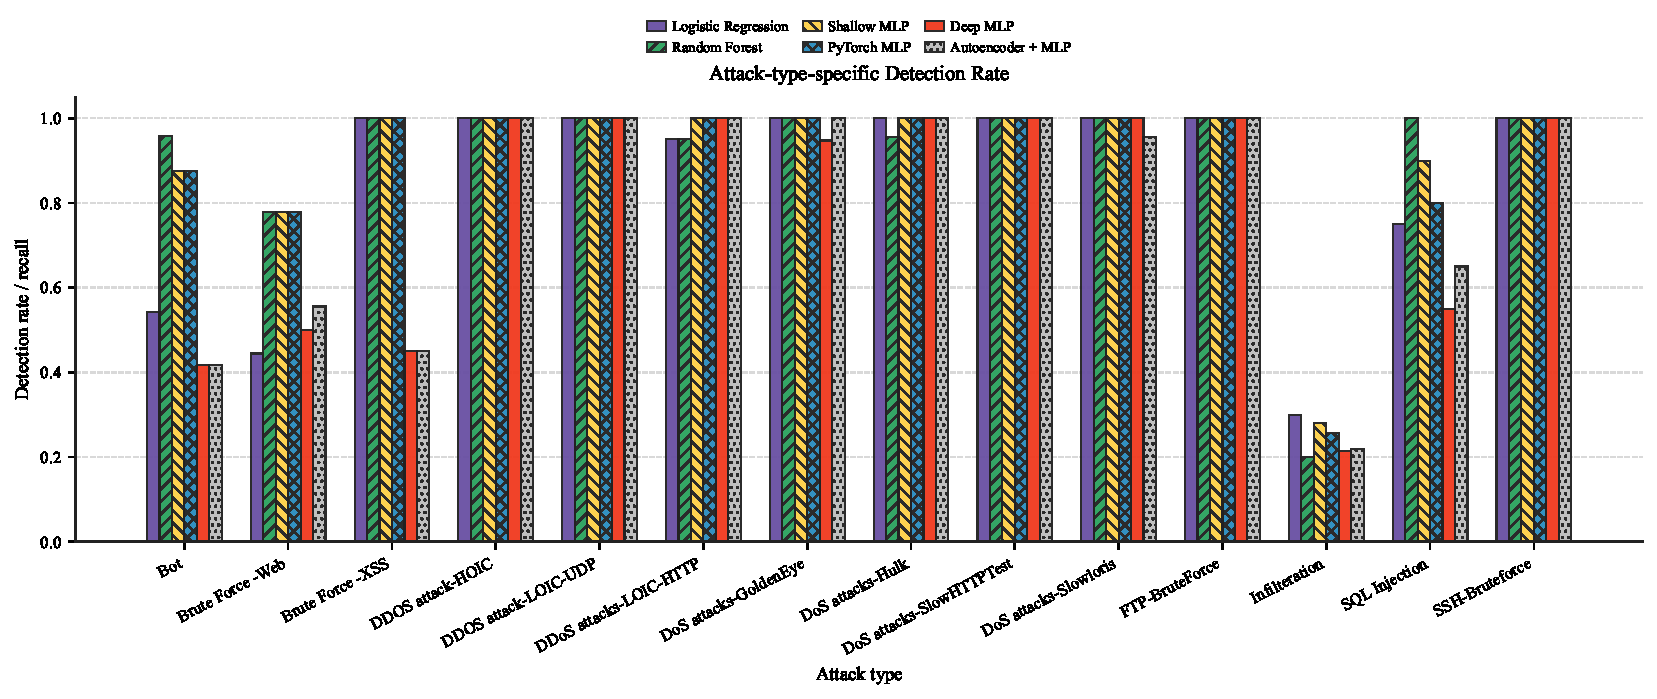
\includegraphics[width=\textwidth]{reports/final_run/attack_type_detection.pdf}
  \caption{Fine-grained attack-type recall by model.}
  \Description{Grouped bar chart showing fine-grained attack-type recall for each model.}
  \label{fig:types}
\end{figure*}

\section{Discussion}

The main lesson is that model choice changes the false-negative distribution more than it simply improves or worsens IDS performance.
The results partially support the hypothesis: Shallow MLP and PyTorch MLP match Random Forest on the Brute Force family, and the MLP models perform very well on DoS/DDoS traffic.
However, neural models do not consistently reduce missed attacks.
The highest-recall model is Logistic Regression, and the lowest-recall models include the deeper neural variants.

This result matters because metric choice changes the conclusion.
If the project reported only F1-score, Deep MLP would look like the strongest model.
If the project reported only precision, Deep MLP would look even better.
But the security objective of an IDS is not only to make accurate malicious predictions.
It is also to avoid allowing malicious traffic to pass undetected.
By that standard, Logistic Regression and Shallow MLP are more attractive than Deep MLP in this experiment.

The attack-type breakdown also shows why aggregate metrics can be misleading.
The experiment shows a concrete mechanism by which aggregate metrics can mislead: strong performance on easier high-signal attacks can coexist with weak coverage of stealthier or more ambiguous attacks.
The fine-grained results separate into three groups.
First, DoS/DDoS and FTP/SSH brute-force traffic are almost solved by these flow-level models.
Second, Bot and SQL Injection favor Random Forest, suggesting that some botnet and web-attack behaviors are captured well by threshold-style rules over tabular flow features.
Third, Infiltration is the unresolved blind spot: it is both frequent and difficult, and every model misses most Infiltration samples.
Across the six models, Infiltration accounts for 96.8\% to 99.5\% of all false negatives.
This turns attack-type-specific evaluation into a diagnostic tool.
Model-specific strengths suggest which traffic patterns a model is biased toward detecting, while shared failures point to dataset, feature, or objective limitations.
For example, Random Forest's strength on Bot and SQL Injection suggests useful threshold-like feature structure, while the shared Infiltration failure suggests that the available flow features or binary objective are insufficient for that attack family.

The operational implication is that choosing the model with the best average score is not enough.
The neural/traditional comparison is therefore best understood as an experimental lens.
Because the models differ in precision, recall, and attack-family behavior, they reveal that aggregate IDS metrics can support one model choice while attack-type false negatives support another.
If only one model had been evaluated, the Infiltration failure could look like a model-specific weakness; by comparing six models, the experiment shows that Infiltration is a shared blind spot while other attack categories depend strongly on model choice.
If the goal is to reduce false alarms, Deep MLP or Autoencoder + MLP may look attractive because they are more precision-oriented.
If the goal is to minimize missed attacks, Logistic Regression and Shallow MLP are safer choices in this experiment.
In practice, the system would need targeted data collection, threshold tuning, or attack-family-specific training for Infiltration before it could be trusted as a broad IDS.
For an operator, the best model depends on whether the priority is fewer alerts or fewer missed attacks in the most relevant attack family.
The same observation also motivates a hybrid IDS design: rather than relying on one global decision rule for all malicious traffic, a system could use attack-family-aware thresholds or combine model signals according to the families each model handles best.

The Autoencoder + MLP result is also informative.
Autoencoders are common in deep IDS literature because they can learn compact representations of high-dimensional flow features.
In this experiment, the autoencoder-based model behaves similarly to Deep MLP: high precision, relatively high F1, but low recall.
This does not prove that autoencoders are ineffective for IDS.
Rather, it shows that this specific latent representation, binary objective, and default threshold did not solve the false-negative problem.
Thus, adding depth or representation learning does not automatically improve security coverage.

\section{Risks and Limitations}

The first limitation is dataset dependence.
CSE-CIC-IDS2018 is a public benchmark dataset, and models may learn dataset-specific artifacts rather than general intrusion behavior.
To reduce this risk, the study avoids accuracy-only reporting and focuses on false negatives by attack type.
However, the results should still be interpreted as behavior on this sampled benchmark, not as a production IDS guarantee.

The second limitation is class imbalance.
Some attack types have small test support, so perfect recall on those labels should not be overclaimed.
For example, several rare attack categories have fewer than 30 test samples.
The analysis therefore gives special attention to Infiltration because it is both frequent and poorly detected.

The third limitation is model tuning.
The neural models were implemented as reproducible baselines rather than exhaustively tuned architectures.
Different thresholds, loss functions, resampling strategies, or hyperparameters might improve recall.
This is especially important because the default 0.5 decision threshold may not be optimal for security.

The fourth limitation is the binary training objective.
The models are trained to distinguish benign from malicious flows, and attack labels are used only after training for analysis.
A multiclass or hierarchical model might learn attack-specific patterns more directly.
The binary design was chosen because it matches a lightweight IDS prototype and keeps the comparison focused.

\section{Future Work}

The first next step is threshold tuning for security objectives.
Instead of using a fixed 0.5 threshold, each model should be evaluated under thresholds chosen to reduce false negatives while controlling false positives.
This would directly test whether Deep MLP and Autoencoder + MLP can trade some precision for better recall.
Reporting precision-recall curves or recall at fixed false-positive budgets would also make the comparison more realistic for an operational IDS, where alert volume is constrained.

The second next step is targeted improvement for Infiltration.
Because Infiltration dominates the missed attacks, future work should inspect its feature distribution, compare it against benign flows, and test whether resampling or cost-sensitive training improves detection.
This is a higher priority than adding more model types because it addresses the main security blind spot.
The goal would be to determine whether Infiltration is difficult because of class imbalance, overlap with benign flow features, sampling artifacts, or the binary training objective.

The third next step is multiclass or hierarchical classification.
A model could first detect malicious traffic and then classify the attack family.
Alternatively, attack-family labels could be used during training to encourage the model to learn category-specific features.
This would test whether attack supervision helps the model learn patterns that are invisible when all malicious flows are collapsed into one positive class.
Another variant is a hybrid ensemble that weights Random Forest more heavily for web and botnet-like traffic, while using MLP-style models for high-volume DoS/DDoS or brute-force traffic.

The fourth next step is broader validation.
The current study uses CSE-CIC-IDS2018.
Running the same pipeline on CICIDS2017 or another flow-level IDS dataset would show whether the attack-specific conclusions generalize beyond one benchmark.
If the same model rankings and blind spots appear across datasets, the conclusion would be stronger; if they change, that would show that IDS model selection is highly dataset-dependent.

\section{Conclusion}

This paper evaluated the limits of aggregate metrics for flow-level intrusion detection and tested whether attack-type-specific analysis can complement them.
In this CSE-CIC-IDS2018 experiment, aggregate metrics alone are not sufficient: neural models do not consistently reduce missed attacks even when some of them improve precision or F1-score.
Deep MLP and Autoencoder + MLP improve precision and F1-score, but Logistic Regression has the highest attack recall and lowest false-negative rate.
Shallow MLP is the most stable neural model by recall and performs close to Logistic Regression.
Thus, the model that looks best by aggregate F1-score is not the model that provides the strongest security coverage.

The strongest conclusion is that IDS evaluation must be attack-type-specific.
Neural models match or slightly improve traditional baselines on some DoS/DDoS and brute-force cases, while Random Forest is stronger on Bot and SQL Injection.
At the same time, Infiltration is difficult for every model: even the best Infiltration recall is only 0.299, and Infiltration accounts for 96.8\% to 99.5\% of false negatives across models.
Therefore, aggregate metrics alone are not just incomplete; they can point to the wrong operational choice.
A model that wins by F1-score may still fail as a security tool if it misses the wrong attack type.
For IDS evaluation, the central question should not be only which model wins, but which attacks remain uncovered after the model wins.
Attack-type-specific analysis also shows which model is useful for which part of the threat landscape, making it a practical basis for model selection rather than just an interpretive add-on.

This changes how the result should be used.
The experiment does not support replacing traditional IDS baselines with deeper neural models simply because they produce better F1-scores.
Instead, it supports a more cautious workflow: choose the model according to the attack families that matter operationally, inspect false negatives by label, and tune the decision threshold around the cost of missed attacks.
The main contribution is therefore not a new highest-scoring IDS model, but evidence that aggregate IDS metrics can mask the attack categories where a model is least secure.
The broader implication is that IDS evaluation should move from model-level leaderboards toward coverage-oriented analysis: a model is not secure because it scores well on average, but because it leaves fewer important attack types uncovered.

\clearpage

\begin{thebibliography}{7}

\bibitem{sharafaldin2018}
[1] I. Sharafaldin, A. H. Lashkari, and A. A. Ghorbani. 2018. Toward Generating
a New Intrusion Detection Dataset and Intrusion Traffic Characterization. In
Proceedings of the 4th International Conference on Information Systems Security
and Privacy, 108--116. https://www.unb.ca/cic/datasets/ids-2017.html

\bibitem{cic2018}
[2] Canadian Institute for Cybersecurity. 2018. CSE-CIC-IDS2018 on AWS: A Realistic
Cyber Defense Dataset. University of New Brunswick. https://www.unb.ca/cic/
datasets/ids-2018.html

\bibitem{breiman2001}
[3] L. Breiman. 2001. Random Forests. Machine Learning 45, 1, 5--32. https://doi.org/
10.1023/A:1010933404324

\bibitem{gamage2020}
[4] S. Gamage and J. Samarabandu. 2020. Deep Learning Methods in Network Intrusion Detection: A Survey and an Objective Comparison. Journal of Network and
Computer Applications 169, 102767.

\bibitem{rosay2020}
[5] A. Rosay, F. Carlier, and P. Leroux. 2020. MLP4NIDS: An Efficient MLP-Based
Network Intrusion Detection for CICIDS2017 Dataset. In Machine Learning for
Networking (MLN 2019), Lecture Notes in Computer Science 12081, 240--254.
https://doi.org/10.1007/978-3-030-45778-5\_16

\bibitem{song2021}
[6] Y. Song, S. Hyun, and Y.-G. Cheong. 2021. Analysis of Autoencoders for Network
Intrusion Detection. Sensors 21, 13, 4294. https://doi.org/10.3390/s21134294

\bibitem{saito2015}
[7] T. Saito and M. Rehmsmeier. 2015. The Precision-Recall Plot Is More Informative
than the ROC Plot When Evaluating Binary Classifiers on Imbalanced Datasets.
PLOS ONE 10, 3, e0118432. https://doi.org/10.1371/journal.pone.0118432

\end{thebibliography}

\end{document}
